\documentclass[12pt,fullpagea4paper,a4paper,doublespace]{article} 
\usepackage{amsmath}
\usepackage{mathtools}
\usepackage{amsfonts}
\usepackage{geometry}
\usepackage{hyperref}%for hyperlink
% \usepackage{multirow}
%\usepackage{booktabs,caption,fixltx2e}
%\usepackage[flushleft]{threeparttable}
%\usepackage{graphicx}
\usepackage[utf8]{inputenc}
\usepackage{color}
\newcommand{\indep}{\rotatebox[origin=c]{90}{$\models$}}
\linespread{1.8}
\addtolength{\evensidemargin}{-.5in}
\addtolength{\oddsidemargin}{-.5in}
\addtolength{\textwidth}{0.8in}
\addtolength{\textheight}{0.8in}
\addtolength{\topmargin}{-.4in}
\usepackage[medium]{titlesec}


\geometry{left=2.5cm,right=2.5cm,top=2.5cm,bottom=2.5cm}



\title{Introduction to Latex}
\author{Zilan Chai}
\date{Oct 05 2021}


\begin{document}
\maketitle

\LaTeX is a tool used to create professional-looking documents. It is based on the WYSIWYM (what you see is what you mean) idea, meaning you only have focus on the contents of your document and the computer will take care of the formatting. Instead of spacing out text on a page to control formatting, as with Microsoft Word or LibreOffice Writer, users can enter plain text and let LATEX take care of the rest.

latex is the mathematical typesetting software


\section{Math}

Lower case Greek letters are written as $\omega$ $\delta$ etc. while upper case Greek letters are written as $\Omega$ $\Delta$.

Mathematical operators are prefixed with a backslash as $\sin(\beta)$, $\cos(\alpha)$, $\log(x)$ etc.


We write integrals using $\int$ and fractions using $\frac{a}{b}$. Limits are placed on integrals using superscripts and subscripts:

\[ \int_0^1 \frac{dx}{e^x} =  \frac{e-1}{e} \]

Subscripts in math mode are written as $a_b$ and superscripts are written as $a^b$. These can be combined an nested to write expressions such as
\[ T^{i_1 i_2 \dots i_p}_{j_1 j_2 \dots j_q} = T(x^{i_1},\dots,x^{i_p},e_{j_1},\dots,e_{j_q}) \]


$\frac{1}{\sqrt{x}}$\\
$$\left(\frac{1}{\sqrt{x}}\right)$$

\begin{equation*}
  1 + 2 = 3 
\end{equation*}
 
\begin{align*}
  1 + 2 &= 3\\
  1 &= 3 - 2
\end{align*}


\begin{align*}
  f(x) &= x^2\\
  g(x) &= \frac{1}{x}\\
  F(x) &= \int^a_b \frac{1}{3}x^3
\end{align*}

$$[
\begin{matrix}
1 & 0\\
0 & 1
\end{matrix}
]$$

$$\left[
\begin{matrix}
1 & 0\\
0 & 1
\end{matrix}
\right]$$

\section{Texts}

Bold, italics and underlining:

\noindent Some of the \textbf{greatest} discoveries in \underline{science}  were made by \textbf{\textit{accident}}.


Comments:
% This line here is a comment. It will not be printed in the document.

Hyperlink:\\
This is my link: \href{https://artofproblemsolving.com/wiki/index.php/LaTeX:Symbols}{LaTeX Symbols}.\\
Another tool: \href{https://www.tablesgenerator.com/}{LaTeX Table Generator}.

    
\noindent    \textcolor{blue}{This text is blue.}\\
    \textcolor{red}{This text is red}
    
    
\section{Adding Pictures}

\begin{figure}[h!]
  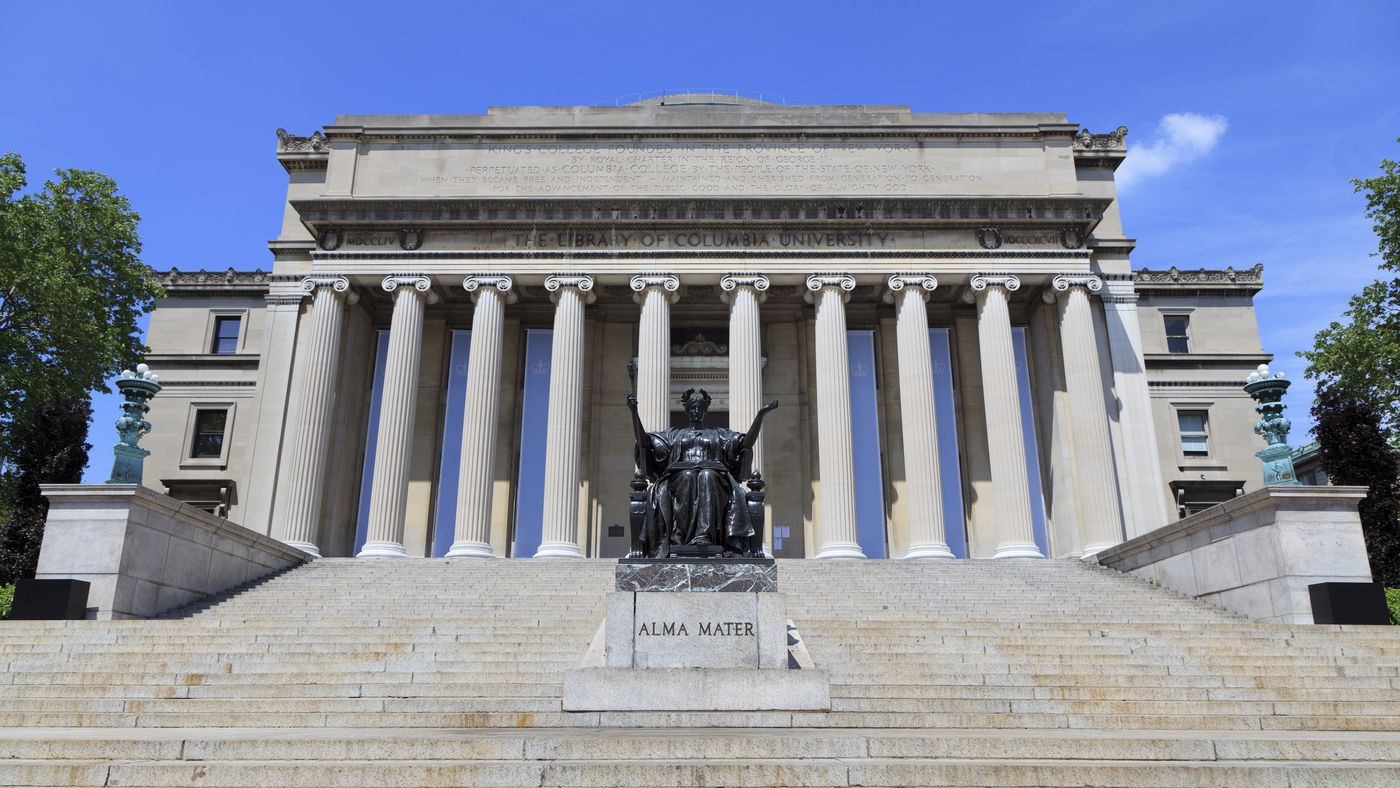
\includegraphics[width=\linewidth]{cu.jpg}
  \caption{Columbia University} 
\end{figure}
https://www.overleaf.com/project/5f6e5c34a9b2b800014ea7be
Image positioning: 

h (here) - same location \\
t (top) - top of page\\ 
b (bottom) - bottom of page\\
p (page) - on an extra page\\
! (override) - will force the specified location\\
 \newpage
\section{Tables}

\begin{table}[h!]
  \begin{center}
    \caption{Your first table.}
    \label{tab:table1}
    \begin{tabular}{l|c|r} % <-- Alignments: 1st column left, 2nd middle and 3rd right, with vertical lines in between
      \textbf{Value 1} & \textbf{Value 2} & \textbf{Value 3}\\
      $\alpha$ & $\beta$ & $\gamma$ \\
      \hline
      1 & 1110.1 & a\\
      2 & 10.1 & b\\
      3 & 23.113231 & c\\
    \end{tabular}
  \end{center}
\end{table}

\section{Sections and Lists}
 
\subsection{This is Section 1}
\begin{itemize}
    \item This is Item 1
    \item This is Item 2

\end{itemize}

\subsection{This is Section 2}
\begin{itemize}
    \item This is Item 2.1 
    \item This is Item 2.2 
\end{itemize}
 
 
\footnotesize

\section{Code}

\begin{verbatim}
library(nnet)
library(VGAM)
library(dplyr)

normal = c(577,192,682,164,145,245)
border = c(27,20,46,4,15,47)
abnormal = c(7,3,11,0,7,27)
age = factor(c(rep("< 40",3),rep("40-59",3)),levels = c("< 40", "40-59"))
smoke = factor(rep(c("never","former","current"),2),levels = c("never","former","current"))
dat = data.frame(normal,border,abnormal, age, smoke)
\end{verbatim}

\end{document}
